%-----------------------------------------------------
% Chapter 3: Descripción del prototipo
%-----------------------------------------------------
\chapter{Desarrollo}

Implementando las prácticas de Lean UX se obtiene: un equipo que trabaja de forma colaborativa, iterativamente y en paralelo, que reduce al mínimo los documentos entregables y que se centra en el software funcional y en el feedback con el usuario. En el capítulo anterior se explican las ideas que subyacen en Lean UX. En esta capítulo se explica en detalle, y de una forma muy práctica, el proceso de implementación de la metodología para el desarrollo del prototipo.


\label{chap: cap3}





\section{Visión, marco y resultados}

Los proyectos de diseño de experiencia de usuario (UX) han estado enmarcados, tradicionalmente, por los requerimientos y las entregas. A los equipos se les suministraban requerimientos para que produjeran entregas. Lean UX cambia por completo este marco de trabajo. El objetivo no es generar un documento entregable, sino producir un resultado. \textbf{No se comienza con requerimientos, sino con suposiciones}. A partir de ellas, se crean y prueban hipótesis. Se mide entonces si, gracias a las hipótesis, se han conseguido alcanzar los resultados que buscábamos. En esta sección se ve la herramienta principal de este nuevo enfoque del trabajo: \textit{las declaraciones de hipótesis}. Estas declaraciones son el punto de inicio del proyecto.\vskip 
Una declaración de hipótesis es una manera de expresar las suposiciones que se tienen del proyecto de una forma comprobable. Está compuesta de los siguientes elementos:

\begin{itemize}
    \item \textbf{Suposiciones}: una declaración de alto nivel que se considera cierta. 
    \item \textbf{Hipótesis}: descripciones más detalladas de las suposiciones dirigidas a áreas específicas de del producto o workflows y con las que es posible experimentar. 
    \item \textbf{Resultados}: el dato de entrada, proveniente del mercado o usuarios, que ayuda a validar o invalidar las hipótesis. A menudo son cuantitativos pero también pueden ser cualitativos. 
    \item \textbf{Personajes}: modelos teóricos de personas para las que se considera estar resolviendo un problema. 
    \item \textbf{Funciones}: los cambios en el producto o mejoras que se consideran que conseguirán los resultados que se buscan.

\end{itemize}

\subsection{Suposiciones}
El primer paso en cualquier proyecto Lean UX es declarar las suposiciones como se puede apreciar en la Figura \ref{fig:leanux1}. Todos los proyectos, no solo los de esta metodología, comienzan de este modo pero, normalmente, no hacen explícitas sus suposiciones. En lugar de ello, se ignoran o, lo que es peor, se tratan como si fueran hechos probados.

\begin{figure}[h]
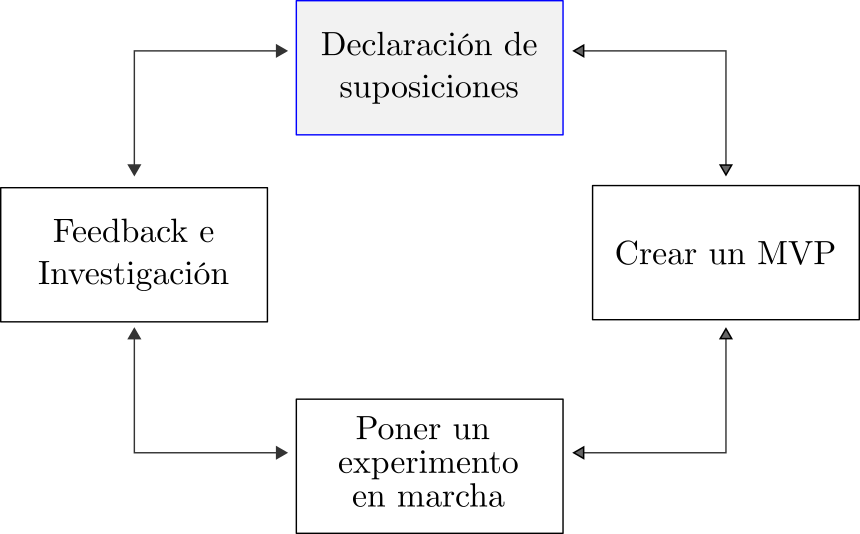
\includegraphics[width=10cm]{Img/Desarrollo/desarrollo1.png}
\centering
\caption{\textbf{ \footnotesize{Proceso LEAN UX, paso 1. }}}
\end{figure}
\label{fig:leanux1}

\subsubsection{Método: declaración de suposiciones}

\textbf{Quién}\vskip
La declaración de suposiciones es un ejercicio que se realiza grupo. Se debe reunir al equipo, asegurándose de que todas las disciplinas estén representadas, e incluye en él a todos los expertos que puedan saber cosas importantes para el proyecto. 

\textbf{Preparación}\vskip
Antes de hacer alguna declaración se debe hacer la preparación recurriendo a técnicas de investigación para recolectar información sobre los usuarios y sus necesidades. El material a preparar antes de iniciar las reuniones puede ser: Informes Analíticos, Análisis de usabilidad, Información sobre intentos pasados para arreglar el problema, investigación de casos similares, etc. 
En la Figura \ref{fig:diagrama-desicion} se puede observar un diagrama de decisión para elegir la técnica de investigación y recolección de información. Se pueden analizar las preguntas:
\begin{enumerate}
    \item \textit{¿Para quiénes se diseña la solución?} La audiencia esta definida por las personas interesadas en los procesos de diseños de productos y no un publico general.
    \item \textit{¿Se conoce el Perfil demográfico del usuario?} Sí: Se considera a las personas mayores de 18 años como potenciales usuarios, por las necesidades propias del ámbito de aplicación.
    \item \textit{¿Es importante el ambiente o locación?} No: Para utilizar la solución no es necesario el ambiente de trabajo o locación del mismo.
    \item \textit{¿Es importante  
    el tiempo o el proceso?} No: El uso de la solución es independiente del tiempo empleado o de las características del proceso que se lleve a cabo.
    \item \textit{¿Se está organizando la información?} No: La organización de la información no es importante, por ejemplo no se organiza en términos de jerarquía o prioridad como se podría organizar un mapa de sitio u organigrama para una institución.
\end{enumerate}
Según las características de este trabajo, la técnica que mejor se adapta es la \textit{entrevista uno-a-uno}\footnote{\url{http://groupquality.com/in-depth-one-on-one-online-interview-techniques/}}. Una vez analizada la información recolectada es necesario declarar el problema de la investigación.



\begin{figure}[h]
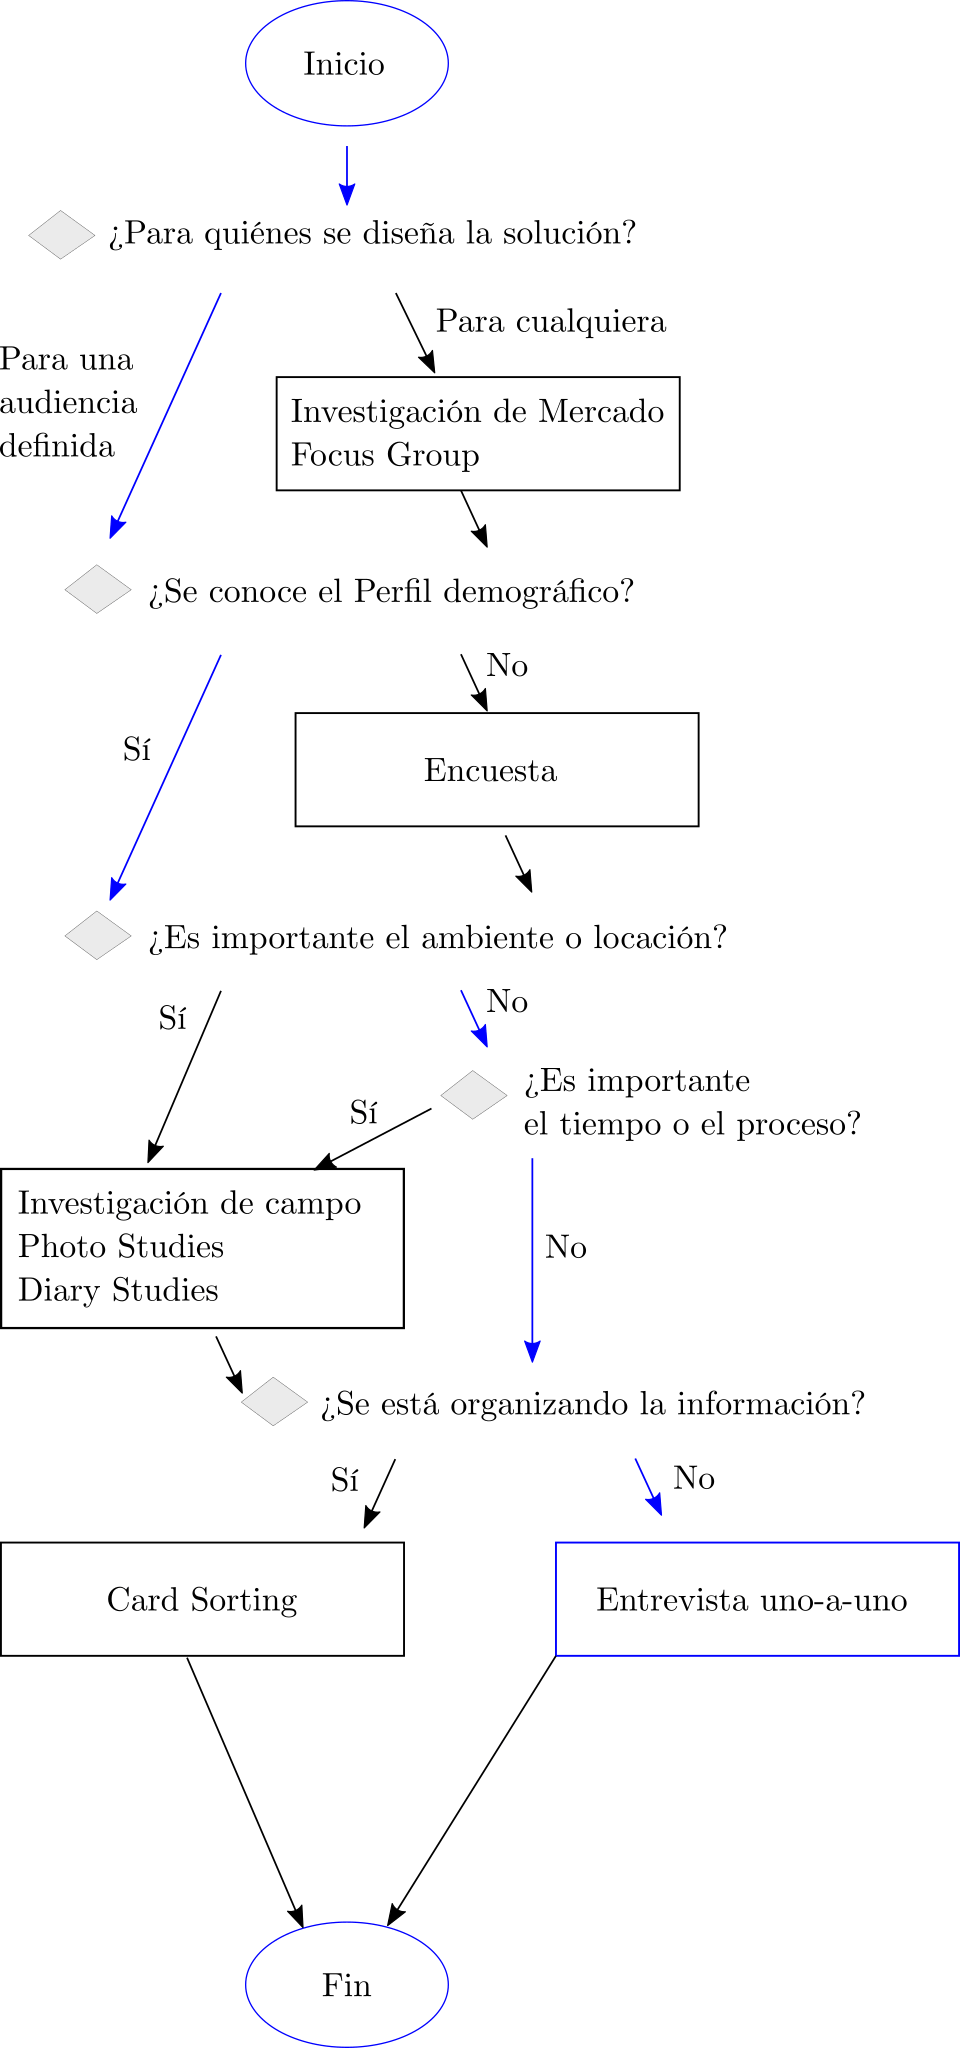
\includegraphics[width=10cm]{Img/CPD/3-flow.png}
\centering
\caption{\textbf{ \footnotesize{Diagrama de desición de investigación del usuario. En los cuadros se especifican las técnicas a utilizar según las desiciones.}}}
\label{fig:diagrama-desicion}
\end{figure}



\subsubsection{Método: declaración de problema}
El equipo necesita un punto de partida para la declaración de suposiciones. Es útil hacerlo con una declaración de problema. La declaración de problema permite centrar correctamente el trabajo de todo el equipo. Además, permite definir las restricciones y límites necesarios para que el equipo trabaje sin perder de vista el objetivo.

Plantilla [Nuestro servicio/ producto] se ha diseñado para cumplir con [estos objetivos]. Sin embargo, hemos observado que no se están alcanzando [estos objetivos], lo que está causando [este efecto adverso] en el negocio. ¿Cómo podríamos mejorar nuestro [servicio/ producto] de modo que nuestros clientes consiguieran mejorar el resultado de su negocio según [estos criterios cuantificables]?\vskip

Nuestro servicio ofrece un canal de comunicación entre aquellos que buscan empleo y los que pueden ofrecérselo. Gracias a él, en nuestro ecosistema los empleadores pueden ofrecer oportunidades de trabajo a los que lo buscan. Hemos observado que un factor crítico que está afectando a la satisfacción de los clientes es la frecuencia de respuesta de los que buscan empleo a los mensajes de los que lo ofrecen. Actualmente, los que buscan empleo están respondiendo a estos mensajes con una tasa muy baja. ¿Cómo podríamos mejorar la eficacia de nuestra comunicación y así conseguir que los que ofrecen empleos tengan más éxito con sus ofertas y los que lo buscan estén más satisfechos con el servicio?\vskip 
Las declaraciones de problema están repletas de suposiciones. El trabajo del equipo es diseccionar las declaraciones de problema y extraer de ellas las suposiciones. Para ello, puedes utilizar la hoja de suposiciones que se presenta a continuación.

\subsubsection{Hoja de Suposiciones}
\label{section:usuarios}

Las suposiciones son una declaración de alto nivel que se considera ciertas.

Todos los proyectos comienzan de este modo pero, normalmente, no hacen explícitas sus suposiciones. En lugar de ello, se ignoran o, en el peor de los casos, se tratan como si fueran hechos probados. En este trabajo se hace hincapié en las \textit{suposiciones de usuarios}, ya que las \textit{suposiciones de negocio} o mercado no intervienen en el desarrollo. A continuación se establecen una serie de preguntas que conforman la \textit{hoja de suposiciones}, con sus respectivas respuestas.


\begin{enumerate}

\item\textbf{¿Quiénes son los usuarios?}
\begin{enumerate}
\item \textbf{Profesionales encargados de crear diseños 3D}. \vskip
Posee las capacidades técnicas y la experiencia sobre procesos y metodologías para llevar a cabo un proyecto de diseño en conjunto con el cliente/usuario.
\item \textbf{Personas sin conocimientos específicos}.\vskip
Desean participar del proceso de diseño pero sin tener conocimientos sobre diseño 3D. Interesados en encargar modelos 3D para la visualización o productos para la fabricación digital. Estas personas pueden ser emprendedores, artistas.
\item \textbf{Personas anónimas}.\vskip
Pueden visualizar los modelos 3D pero no participan en los procesos de diseño.
\end{enumerate}

\item{\textbf{¿Cómo encajaría el producto en su trabajo?}}

\begin{enumerate}

\item Sería excelente poder visualizar el producto en la web.

\item De manera positiva aunque un poco arriesgada por el cambio de paradigma.

\item Provocaría rechazo por personas con poca organización.

\item Positivo, sería muy interesante ver la organización de los diseños y el proceso.\vskip

\item Sería muy positivo si permite no depender tanto del email.\vskip

\end{enumerate}

\item{\textbf{¿Qué problemas soluciona el producto?}}

    \begin{enumerate}
    
    \item La visualización de un modelo 3D en proceso. \vskip
    
    \item Soluciona el diseño completo para personas que no saben de modelado 3D. \vskip
    
    \item La comunicación para discutir sobre un producto.\vskip
    
    \item La organización de los modelos y el progreso.\vskip
    
    \item Llevar un registro sobre los pagos y entregas.\vskip
    
    \end{enumerate}


\item{\textbf{¿Cuándo y cómo se utilizaría el producto?}}
    \begin{enumerate}
    \item En cualquier momento y en cualquier lugar, desde cualquier dispositivo con internet. \vskip
    
    \item En el lugar de trabajo en una intranet, así nadie puede ver los diseños.\vskip
    
    \item En cualquier momento y desde un dispositivo moderno.\vskip
    
    \item Sólo se utilizaría cuando se esté de viaje.\vskip
    
    \item Sólo desde la PC, sino es muy incómodo ver algo.\vskip
    
    \end{enumerate}


\item{\textbf{¿Cuáles serían las funciones más importantes?}}

    \begin{enumerate}
    \item Poder ver un modelo con muchos detalles, girarlo, agrandarlo, etc. \vskip
    
    \item Poder hacer cambios drásticos en los modelos sin necesidad de saber de 3D.\vskip
    
    \item Poder registrar los pagos para que haya transparencia.\vskip
    
    \item Poder comunicarse con el Diseñador y hacer feedback en una especie de chat.\vskip
    
    \item Poder hacer anotaciones en los modelos para que la otra persona vea. \vskip
    
    \item Tener registro de los pedidos de cambio con fecha y hora.\vskip
    
    \item Poder agregar documentos como planos, contratos.\vskip
    
    \item Poder ver como interactúa el producto con su entorno, por ejemplo en un paisaje o en un diseño de interiores.\vskip
    
    \item Poder ver con realidad virtual, con efectos realistas.\vskip
    
    \end{enumerate}

\item{\textbf{¿Qué aspectos debe tener y cómo debe comportarse?}}

    \begin{enumerate}
    \item Debe ser bonito y fácil de usar. \vskip
    
    \item Debe ser parecido a los programas de CAD con mucha opciones y muy rápido.\vskip
    
    \item No importa si es bonito, lo importante es que funcione bien y rápido.\vskip

    \item Debe ser agradable a la vista y fácil de usar como una red social.\vskip
    \end{enumerate}

\end{enumerate}

\subsubsection{Priorización de las suposiciones} 
Las suposiciones se declaran al inicio del trabajo para poder identificar los riesgos del proyecto. Una vez que se dispone de la lista de suposiciones se necesita averiguar cuáles de ellas tienen más riesgo. Lean UX lleva a cabo un ejercicio implacable de priorización, una vez que se comprende que no se pueden probar todas las suposiciones del proyecto, la cuestión que se presenta es: \textit{¿cuál de ellas se debe de probar primero?} \vskip
Para decidir sobre esta cuestión, se puede crear un gráfico como el que aparece en la Figura \ref{fig:priori} y situar en él la lista de suposiciones. El objetivo del gráfico es decidir qué suposiciones se debe probar primero, en base a:
\begin{enumerate}
    \item \textbf{El nivel de riesgo} \vskip
    Por ejemplo, si se hiciera esto mal, ¿hasta qué punto se vería perjudicado el proyecto?
    \item \textbf{El conocimiento que se tenga de la suposición}.\vskip
    Por ejemplo, un caso típico es la función para acceso de usuario o \textit{login}, esta suposición es bien conocida o por lo menos un mecanismo muy utilizado por la mayoría de los usuarios.
\end{enumerate}
 Cuánto más alto sea el riesgo que implica una suposición y menos se sepa de ella, mayor debe ser la prioridad. La asignación de la prioridad para la prueba no significa, ni mucho menos, que aquellas que no sean prioritarias desaparezcan del proyecto para siempre. Es recomendable mantener una lista de cuestiones pendientes con las suposiciones que no se hayan priorizado para poder volver a ellas y probarlas si se demuestra que amerita hacerlo.


\begin{figure}[h]
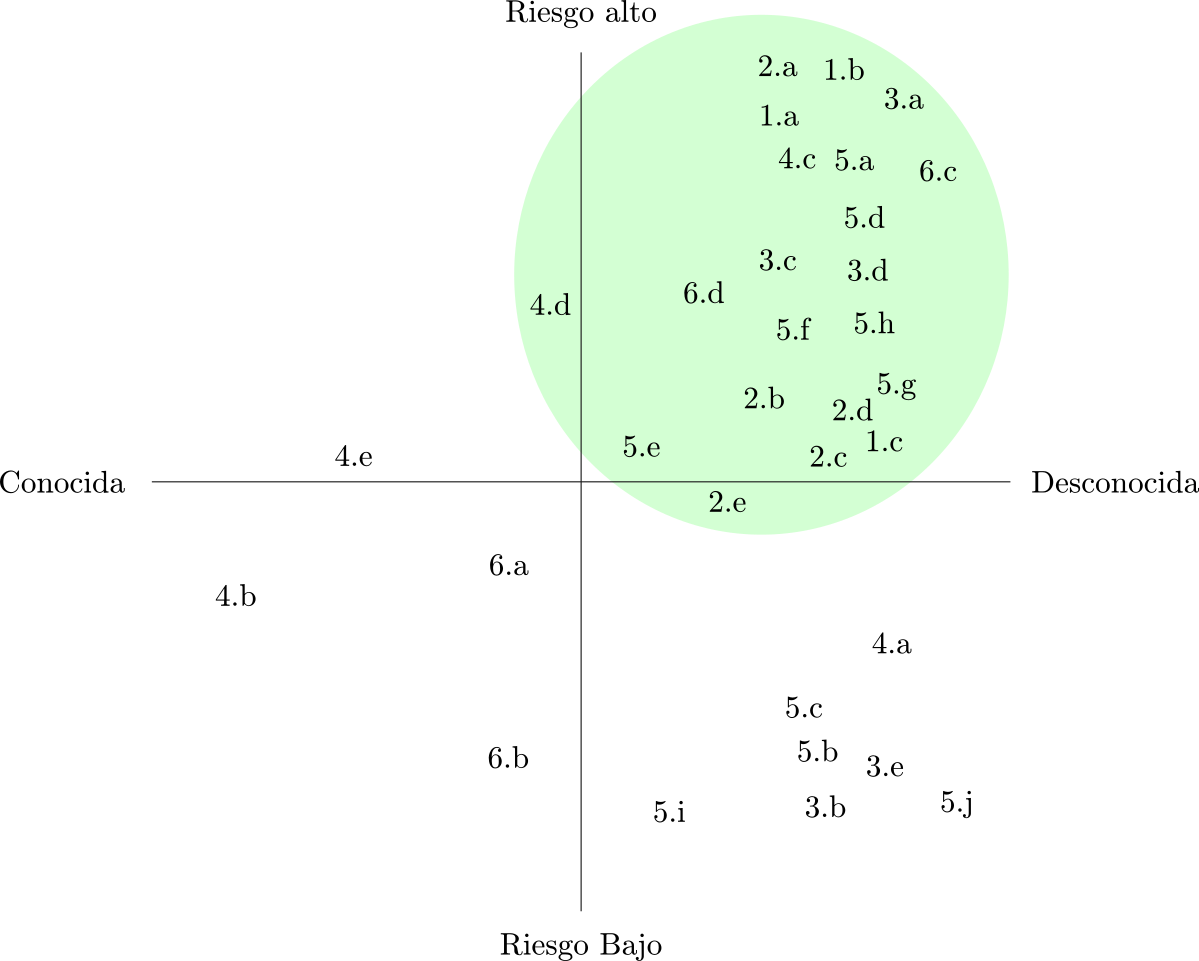
\includegraphics[width=14cm]{Img/Desarrollo/desarrollo-matriz.png}
\centering
\caption{\textbf{ \footnotesize{ Matriz de priorización de suposiciones }}}
\label{fig:priori}
\end{figure}

Para comprender las asignaciones de prioridad, a continuación se explican algunas suposiciones. 

En la zona superior derecha de la matriz se pueden apreciar las suposiciones con mayor prioridad. Por ejemplo: 

\begin{itemize}

    \item \textbf{1.b Personas sin conocimientos específicos en 3D}\vskip
    El riesgo de no probar esta suposición es alto, ya que la posibilidad de participación de este tipo de usuario es un valor fundamental para la aplicación. 
    \item \textbf{2.a Sería excelente poder visualizar el producto en la web}\vskip
    Si no se prueba esta suposición el proyecto fracasa porque el uso de modelos en la web es un requisito indispensable para el funcionamiento de la aplicación.
    \item \textbf{6.c No importa si es bonito, lo importante es que funcione bien y rápido}\vskip
    En esta suposición se pueden percibir aspectos de experiencia de usuario, probarla ayudaría a conocer la aceptación del usuario. Por ende, esta suposición implica un riesgo enorme porque es prioritaria la aceptación del usuario en el uso de la aplicación.
\end{itemize}

Fuera de la zona verde de la matriz se pueden apreciar las suposiciones con menor prioridad. Por ejemplo: 

\begin{itemize}

    \item \textbf{5.j Poder ver con realidad virtual, con efectos realistas.}\vskip
    Si no se prueba esta suposición, el proyecto no corre riesgo de continuar ya que no es un requisito indispensable, por otro lado el grado de desconocimiento sobre el tema es elevado en el contexto de este trabajo.
    \item \textbf{4.e Sólo desde la PC, sino es muy incómodo ver algo}\vskip
    La prueba de esta suposición, limitando la aplicación a ese tipo de dispositivos no pone en riesgo el proyecto, ya que la mayoría de los usuarios también utilizan dispositivos móviles y para los objetivos del proyecto no tendría sentido el gasto para desarrollar la prueba.
   
\end{itemize}



\clearpage
\subsubsection{Hipótesis}
Cuando se obtiene la lista de suposiciones priorizada, se puede dar el siguiente paso: \textbf{probarlas}. Para hacerlo, es necesario transformar cada declaración de suposición a un formato más sencillo de probar: \textit{Una descripción general de lo que se debe hacer y que impacto se espera}.\vskip


Ejemplo: \textbf{Desarrollando una solución de comunicación de diseños de productos para un equipo multidisciplinario se logrará una mayor tasa de participación y un aumento en la satisfacción de los involucrados.}

\subsubsection{Subhipótesis: división de las hipótesis en partes más pequeñas }
La hipótesis planteada anteriormente es demasiado extensa para que, con una única prueba, pueda determinarse su validez. Esto se produce porque la hipótesis contiene demasiadas partes móviles, es decir, demasiadas subhipótesis. Cuando esto sucede, se recomienda dividir las hipótesis en partes más pequeñas y específicas. Para el trabajo de desarrollo de productos en particular se puede utilizar el siguiente formato: \vskip
\textbf{Se considera que [haciendo esto - desarrollando esta función - creando esta experiencia de usuario] para [estas - personas - personajes] se conseguirá [este resultado]. 
Se sabrá si esto es correcto cuando se obtenga [este feedback del entorno o mercado, esta medida cuantitativa, o este conocimiento cualitativo]}\vskip El primer campo se completará con la función o mejora que está considerando para el producto. El segundo describirá exactamente qué usuarios objetivo se beneficiarán de la función. El último campo, por su parte, especifica los beneficios que esos usuarios obtendrán de ella. La frase final lo une todo. Esta frase determina si la hipótesis es cierta o no.\vskip
¿Qué resultado del feedback con el entorno será el que indique que la idea es correcta? Podría ser una medida cuantitativa, como el uso que hacen los usuarios de una determinada función del producto, por ejemplo, o como el incremento de una métrica de negocio, o bien una medida cualitativa, por ejemplo el grado de satisfacción en el uso.


DEFINIR ESTOOOOOOOOOOOOOOOOOOOOO
\textbf{Se considera que desarrollando una solución de comunicación de diseños de productos para un equipo multidisciplinario, logrará una mayor tasa de participación y un aumento en la satisfacción de los involucrados.
Se verificará que esto es cierto cuando aumenten las opiniones de los involucrados y se pueda registrar la evolución del diseño.}
\vskip

Para crear las declaraciones de hipótesis, se comienza por el principio. Se recomienda tener una lista de los resultados que quieres provocar, la definición de los personajes a los que se pretendes dar servicio y el conjunto de funciones que se considera que podrían funcionar bien en esta situación. Una vez que se dispone de todo este material, se puede obtener un conjunto de declaraciones.


\subsubsection{Resultados}
En la creación de las hipótesis que se quieran probar, se debe ser específico respecto a los resultados que se pretendes obtener. Los equipos Lean UX están menos centrados en los documentos de salida (los documentos, esquemas e incluso los productos y funciones que produzcamos) y más en los resultados reales que esos documentos generan: Ej. ¿se puede conseguir que la gente se conecte se manera sencilla a la aplicación? ¿Cómo convencerlos de que se den de alta en el servicio? ¿Se puede animar a los usuarios del sistema a que colaboren más entre ellos? Junto con el equipo, considera el problema que tratas de resolver. Probablemente contarás con unos cuantos resultados de alto nivel que esperas obtener (por ejemplo, un aumento en los usuarios registrados en la página, un aumento del uso, etc.). Considera ahora cómo podrías dividir esos resultados en componentes más pequeños. ¿Qué comportamientos podrían predecir un mayor uso de la página?: ¿un mayor número de visitas o un mejor comportamiento del click-through en los correos de marketing? ¿O tal vez un aumento en el número de artículos en la cesta de la compra de la página? A veces es útil realizar una sesión de brainstorming con el equipo para establecer qué resultados individuales, tomados en conjunto, pueden contribuir a conseguir el resultado total.

\begin{figure}[h]
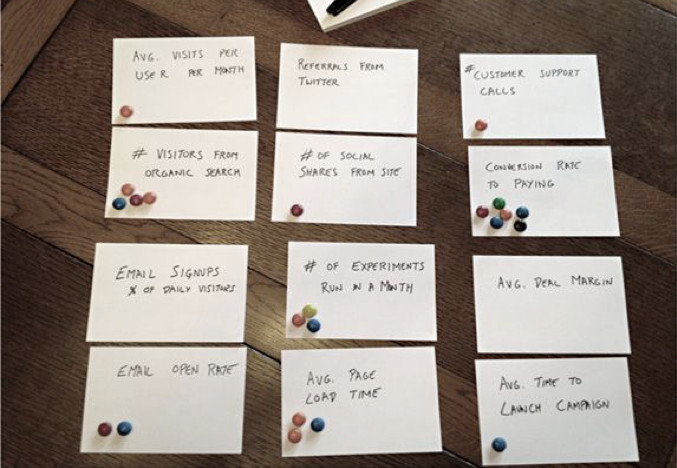
\includegraphics[width=12cm]{Img/Desarrollo/desarrollo2.jpg}
\centering
\caption{\textbf{ \footnotesize{ Priorización de KPI con caramelos }}}
\label{fig:priori}
\end{figure}

La figura 3-3 muestra un ejemplo de Giff Constable, en él se ve el resultado de una sesión de brainstorming realizada por un equipo de liderazgo ejecutivo, que votó cuáles deberían ser los siguientes KPI (Key Performance Indicators, indicadores clave de rendimiento) que la compañía tendría que cumplir. Después de recopilar los resultados de la votación en la lista de indicadores que se puede ver en la fotografía, a cada ejecutivo se le dieron 4 M& M. En lugar de comérselos, cada uno de ellos los utilizó para votar por la métrica que consideraban más importante. De esta manera, el CEO consiguió acabar con la discusión.


\subsubsection{Personajes}

Los diseñadores crean a menudo modelos, denominados personajes, para representar a los usuarios de sus sistemas. Si el equipo ya dispone de un conjunto de personajes bien definido, solo se debe que decidir cuáles de ellos se emplearán para confirmar las declaraciones de hipótesis. Si aún no se dispone de ellos, a continuación se explica cómo crearlos para el proceso Lean UX.

\vspace{5mm}
\textbf{Proto-Personajes}\vskip
En lugar de emplear meses enteros realizando trabajo de campo y entrevistando a personas, se dedican unas horas a la creación de lo que se denominan \textit{protopersonajes}, modelos que detallan quién utilizará nuestro producto y por qué lo hará. Se parte de un modelo muy esquemático, en cuya creación participa todo el equipo. A medida que se avanza en la investigación y se aprende más sobre los usuarios del producto, se pueden ajustar tanto el publico objetivo como el diseño.

\begin{figure}[h]
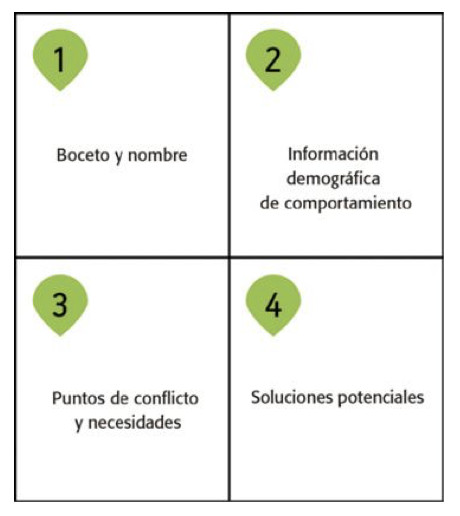
\includegraphics[width=10cm]{Img/Desarrollo/desarrollo-blanco.jpg}
\centering
\caption{\textbf{ \footnotesize{Proto-persona del profesional}}}
\end{figure}

\begin{figure}[h]
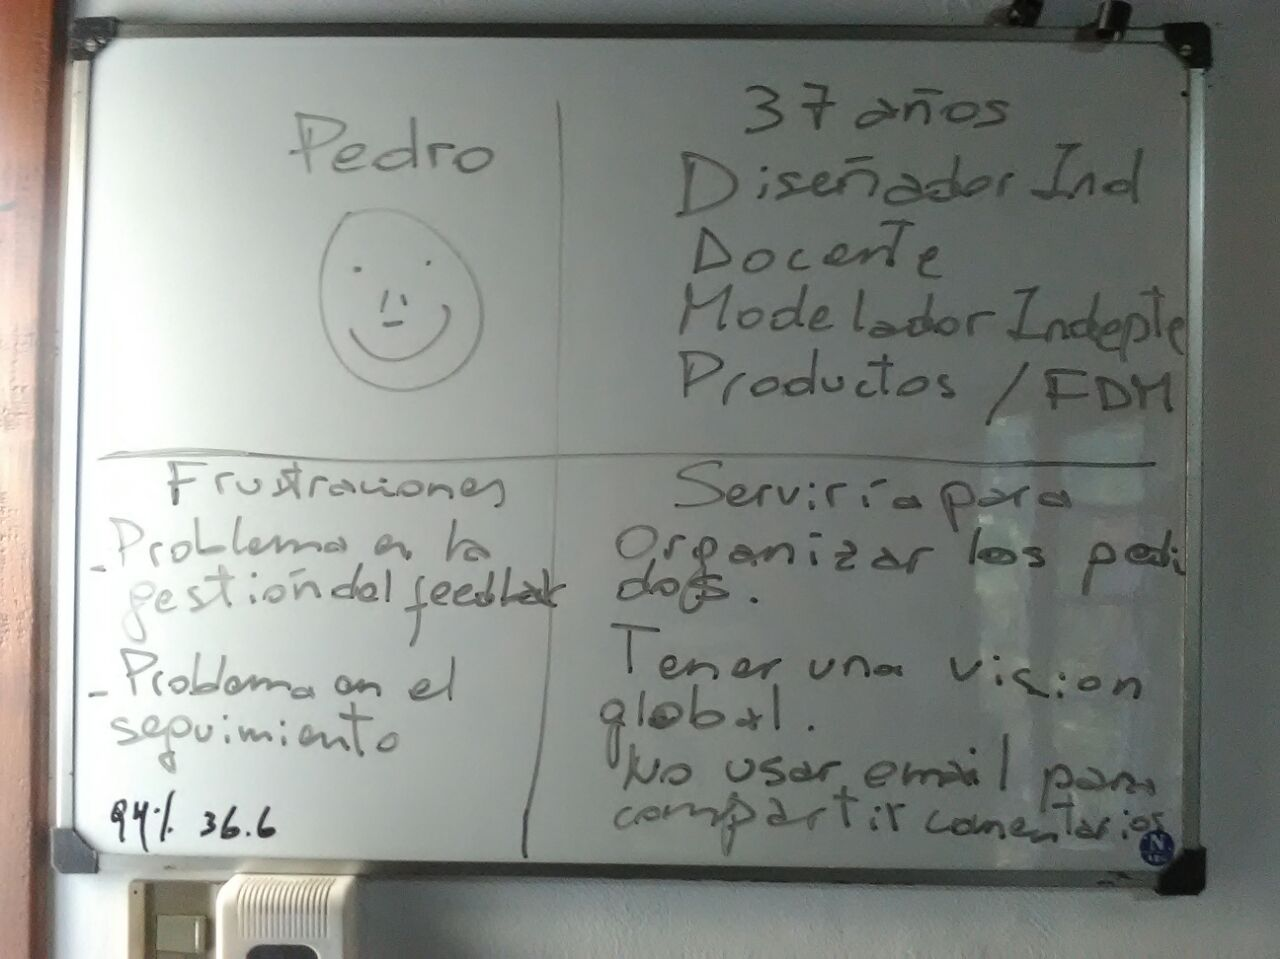
\includegraphics[width=10cm]{Img/UX/UX-proto.jpg}
\centering
\caption{\textbf{ \footnotesize{Proto-persona del profesional}}}
\end{figure}

\textbf{Formato de Proto-personaje}\vskip
En la mitad inferior del esquema, se situa la parte más importante de la información. El cuadrante inferior izquierdo debe contener las necesidades de los usuarios y las frustraciones que hayan podido experimentar con la solución actual, los puntos de conflicto específicos que el producto está tratando de resolver y/ o la oportunidad que se trata de capturar con él. El cuadrante inferior derecho contiene las soluciones potenciales para esas necesidades. En este cuadrante se incluye las soluciones y las funciones que se consideren.


\subsubsection{Funciones}
 Una vez que se obtiene una lista de resultados en mente y se enfoque en un grupo de usuarios concreto, se comienza a comenzar a pensar en las técnicas, las funciones, los productos y los servicios a desarrollar para conseguir esos resultados. Normalmente, en este punto todos los miembros del equipo tendrán su propia opinión sobre el tema, ya que, después de todo, las funciones son lo más concreto con lo que han trabajado, por lo que les resultará más sencillo expresar sus ideas en términos de funciones. Sin embargo, un error común es hacer que el proceso de diseño parta de ellas: alguien tiene una idea sobre una función a implementar y, al final, todo el equipo intenta cubrir las etapas iniciales en el orden incorrecto para justificar esa función. Se debe recordar que, en Lean UX, las funciones existen para satisfacer las necesidades del negocio, del cliente y de los usuarios.


\textbf{Organización de las subhipótesis}\vskip

Con todo el material en bruto obtenido, se puede organizar en hipótesis que puedan probarse. Se puede usar una tabla como la de la tabla XXX. Se debe tener en cuenta, a medida que se escriban las hipótesis, a qué personajes sirven las soluciones propuestas. Es posible que algunas soluciones sirvan a más de un personaje. Si las hipótesis producen más de un resultado, se pueden dividir la hipótesis en varias partes, ya que cada declaración debe referirse a un único resultado. Es importante recordar que ideas deben ser lo suficientemente específicas, para crear pruebas significativas que las puedan validar.



\begin{tabular}{ |p{1cm}|p{3.5cm}|p{4.5cm}|p{4.5cm}| }

\hline
    Núm. & Se desarrolla & Para  & Para\\
\hline
1 & Un visualizador de modelos 3D & Para la persona con rol diseñador experto (XXX) & que solucione la visualización online de los avances de su trabajo \\
\hline
2 & Un visualizador de modelos 3D & Para la persona con rol diseñador experto (XXX) & que solucione la visualización online de los avances de su trabajo \\
\hline
\end{tabular}

- Ingreso / Modificación de parámetros
- Visor de historias / notas / chat
- Almacenamiento de archivos relacionados


Una vez obtenida la lista de hipótesis, se puede avanzar al siguiente paso. Esta lista sirve como una guía para el próximo paso en el proceso Lean UX: el \textit{diseño colaborativo}.

\clearpage
\section{Diseño Colaborativo}
Lean UX es un proceso colaborativo que reúne a diseñadores y no diseñadores (programadores, administradores de proyectos) en un trabajo de creación conjunta para crear los conceptos del producto. También les ayuda a construir un entendimiento común sobre el problema y sobre las soluciones de diseño. Asimismo, les permite decidir qué funcionalidad y elementos de la interfaz implementan mejor las funciones recogidas en las hipótesis. La documentación de salida de las sesiones de diseño consta normalmente de esquemas de baja fidelidad y \textit{wireframes}. Es escencial que la documentación inicial no sea muy elaborada para que el trabajo continúe siendo maleable. De esta manera, el equipo puede cambiar de dirección con facilidad una vez que sus pruebas les demuestren que el enfoque adoptado no funciona. A continuación se describen algunas herramientas utilizadas para el diseño del prototipo.

\subsection{Estudio de diseño}
El equipo se reúne en una sesión de trabajo o \textbf{Estudio de Diseño} (a veces también llamado Charrette de diseño)\citep{Gothelf2013}. Es una manera de conseguir que un equipo multidisciplinario visualice de forma conjunta las soluciones potenciales a un problema de diseño. Se usan técnicas específicas para llevar a cabo las sesiones de Estudio, dependiendo de la situación del proyecto y los plazos de entrega. Abarca los siguientes pasos:
\begin{itemize}
    \item Definición del problema y sus restricciones. 
    \item Generación de ideas individuales (divergir). 
    \item Presentación y críticas. 
    \item Iteración y perfeccionamiento (emerger). 
    \item Generación de ideas del equipo (converger).
\end{itemize}


\begin{figure}[h]
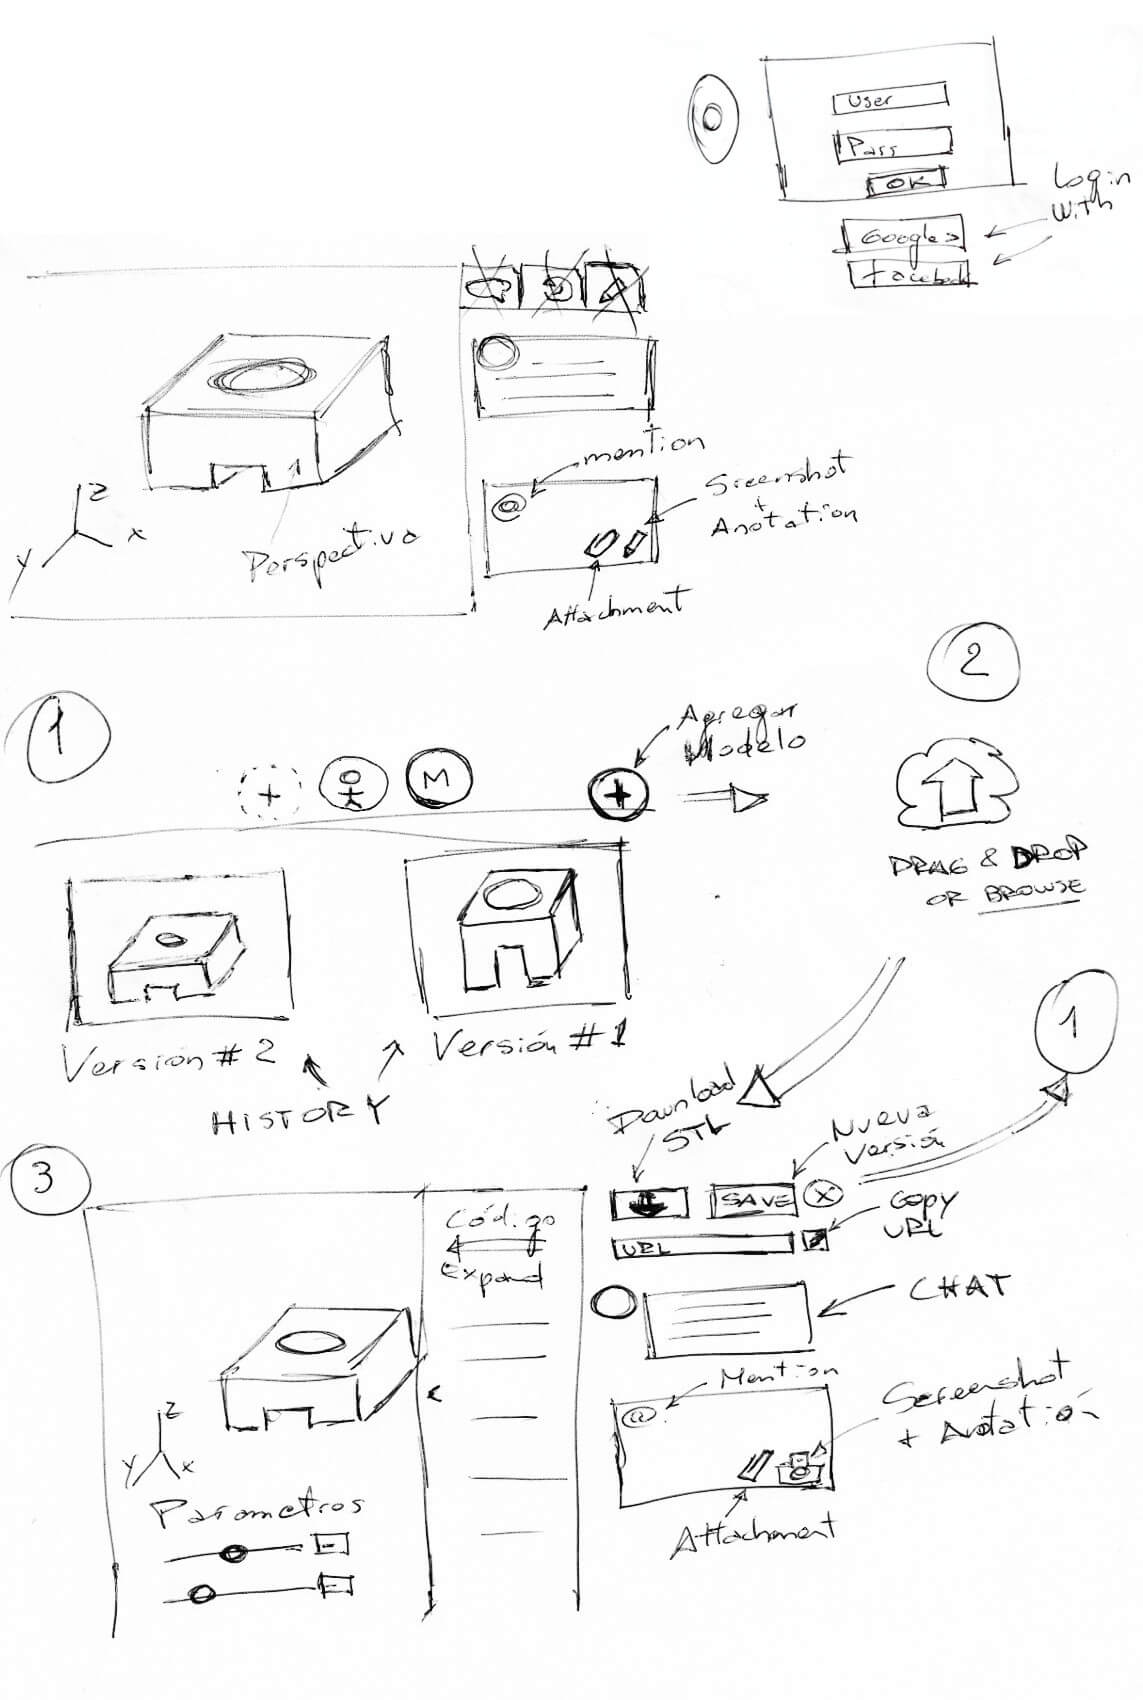
\includegraphics[width=14cm]{Img/UX/edc.jpg}
\centering
\caption{\textbf{ \footnotesize{Sketch de Interfaces como salida del estudio de diseño}}}
\end{figure}


\begin{figure}[h]
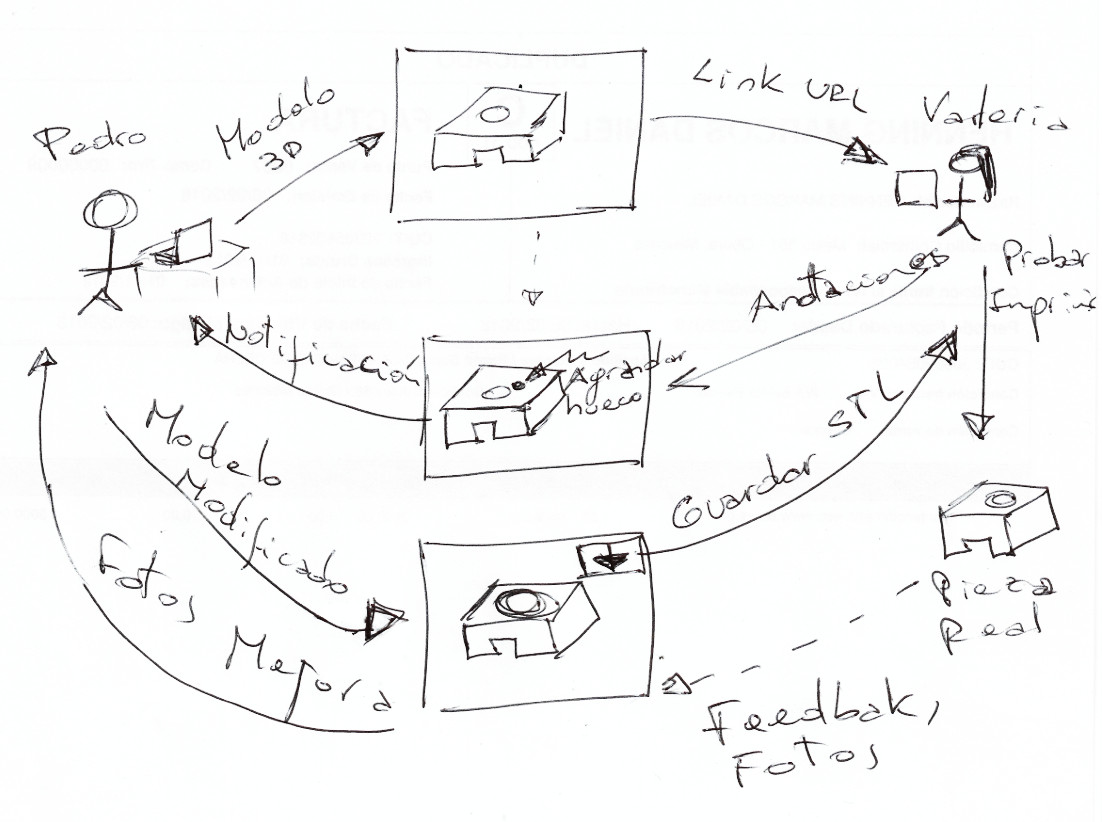
\includegraphics[width=14cm]{Img/UX/ed2.jpg}
\centering
\caption{\textbf{ \footnotesize{Posibles escenarios diseñados en el estudio de diseño}}}
\end{figure}

Los resultados del estudio de diseño se realizan comúnmente utilizando Lápices, Bolígrafos, Marcadores (de varios colores). Plantillas para esquemas, Pegatinas.

El objetivo del estudio del diseño es preparar todo el material para el siguiente paso de Lean UX: \textit{crear un PMV y probarlo con un experimento}.


\clearpage
\subsection{Definición de Componentes y Guía de estilo}
Una herramienta que facilita el diseño es la \textbf{guía de estilo}, \textit{una biblioteca de patrones aceptada por todo  el equipo, que codifica los elementos gráficos e interactivos de una interfaz de usuario. También sirven para recopilar todos los componentes del producto a los que se enfrentará el usuario, todo lo que forme parte de la experiencia del usuario aparece en la guía de estilo.} Algunas empresas utilizan \textit{wikis} para la guía de estilo, lo que permite que toda la colección permanezca actualizada y que esté disponible para el equipo. Otros prefieren crear guías de estilo ``dinámicas", es decir, repositorios de diseño y de código front-end\footnote{Front-end es la parte del software que interactúa con los usuarios.} que no solo definen el aspecto y el comportamiento del producto, sino que también proporcionan el lenguaje necesario y las hojas de estilo en inglés \textit{Cascading Style Sheet} (CSS)\footnote{\url{https://www.w3.org/Style/CSS/}} para la interfaz de cliente. De esta manera, al modificar la guía de estilo también se modifica el producto.
Para la estética del prototipo COCADA se eligió el concepto de diseño \textit{Material Design}\footnote{\url{https://material.io/guidelines/}}, un diseño donde la profundidad, las superficies, los bordes, las sombras y los colores juegan un papel principal. A continuación se especifican algunos componentes gráficos y diseños a utilizar:


\subsubsection{1. Tamaños de letras según dispositivos}
    \begin{figure}[h]
    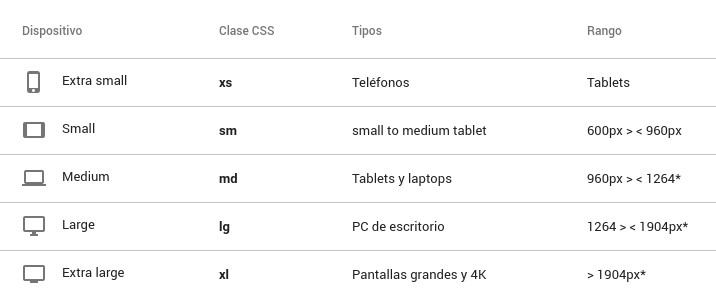
\includegraphics[width=14cm]{Img/UX/guia1.jpg}
    \centering
    \caption{\textbf{ \footnotesize{Tamaño de letras con sus respectivas clases CSS}}}
\end{figure} 
    
\subsubsection{2. Esquema de colores}
\begin{figure}[h]
    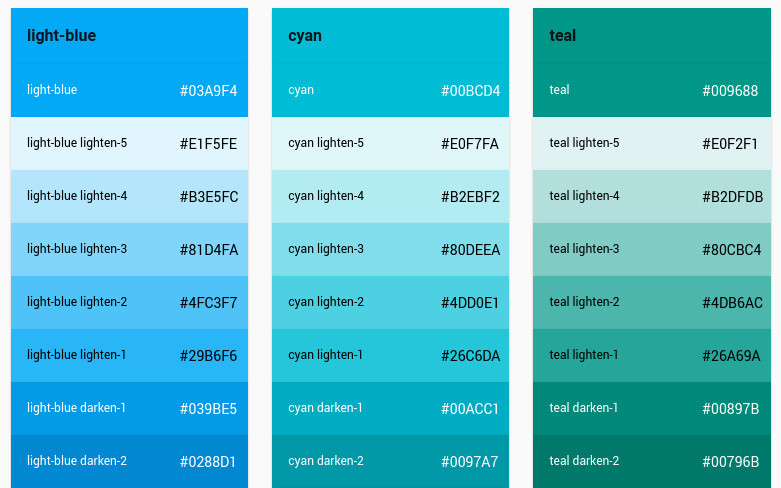
\includegraphics[width=12cm]{Img/UX/guia0.jpg}
    \centering
    \caption{\textbf{ \footnotesize{Esquema de colores con sus respectivas clases de CSS}}}
\end{figure}


\subsubsection{3. Iconos mediante fuentes tipográficas}
    Usando el prefijo fa- seguido del nombre del ícono como clase CSS. Las fuentes tipográficas son vectoriales, por lo que se puede cambiar el tamaño y color de los iconos sin perder calidad.
    \begin{figure}[h]
    
\includegraphics[width=11cm]{Img/UX/guia3.jpg}
    \centering
    \caption{\textbf{ \footnotesize{Iconos mediante fuentes tipográficas. Clase de CSS ej: .fa-email}}}
   
    \end{figure}
    
 
\subsubsection{4. Botones de acción simples}
    \begin{figure}[h]
    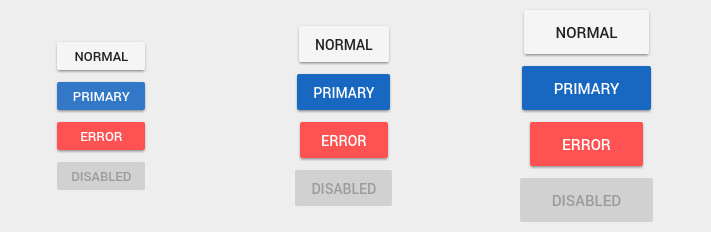
\includegraphics[width=11cm]{Img/UX/guia2.jpg}
    \centering
    \caption{\textbf{ \footnotesize{Estilos de botones. Clase de CSS ej: .btn.primary}}}
    \end{figure}
    
\clearpage
\subsubsection{5. Botones de acción flotante}\vskip
El Botón de Acción Flotante (FAB) es un botón circular con un ícono flotando en una página. El propósito de un FAB es parecido a un botón llamado-a-la-acción en ingles \textit{call-to-action}\footnote{\url{https://en.wikipedia.org/wiki/Call_to_action_(marketing)}}; enfatiza una acción que la mayoría de los usuarios presumiblemente realizaría. Generalmente se presenta con un color vívido que lo hace más prominente entre el resto de los elementos de la aplicación.
    \begin{figure}[h]
    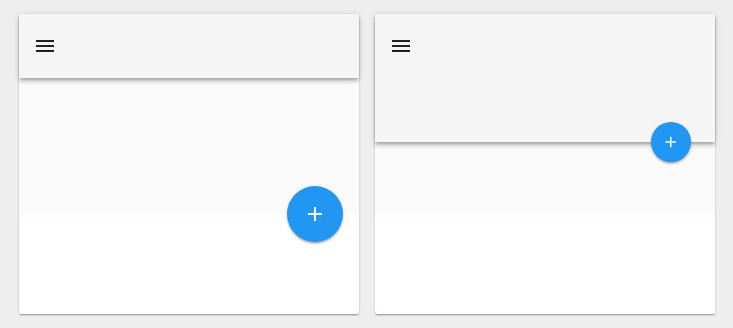
\includegraphics[width=12cm]{Img/UX/guia4.jpg}
    \centering
    \caption{\textbf{ \footnotesize{Botones de acción flotantes. Clase de CSS ej: .btn-floating.blue}}}
    \end{figure}
    

\subsubsection{6. Controles de entrada}\vskip
Estos elementos sirven para ser usados de múltiples formas. En el prototipo se utilizan sobre todo para la manipulación de parámetros de los modelos 3D y  también para la mayoría de los formularios.
    \begin{figure}[h]
    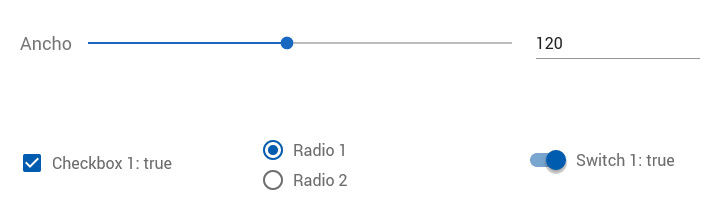
\includegraphics[width=14cm]{Img/UX/guia6.jpg}
    \centering
    \caption{\textbf{ \footnotesize{Controles gráficos.}}}
    \end{figure}



\clearpage  
\subsubsection{7. Cards o Tarjetas}\vskip
Las Tarjetas se están convirtiendo rápidamente en un patrón de UI indispensable, particularmente para las webs móviles. Esto se debe en parte a las webs como Pinterest\footnote{\url{https://pinterest.com}} y Twitter que hacen uso exhaustivo de las mismas. En el prototipo se utilizan tarjetas para listados o grillas de modelos que son parte de un proyecto.
    \begin{figure}[h]
    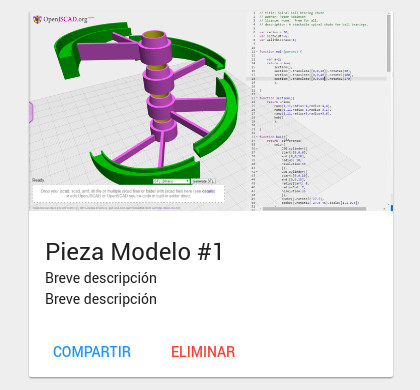
\includegraphics[width=7cm]{Img/UX/guia5.jpg}
    \centering
    \caption{\textbf{ \footnotesize{Tarjeta de un modelo 3D}}}
    \end{figure}
    
\subsubsection{8. Comentarios}\vskip
En el prototipo, los comentarios se pueden considerar tarjetas con un formato específico. Sirven para definir listados de comentarios o hilos de conversaciones, que hacen posible la comunicación entre los participantes de un proceso de diseño. Se pueden apreciar en la Figura \ref{fig:comment} el uso de hashtag (\#) y menciones (@), como en la mayoría de las redes sociales.
    \begin{figure}[h]
    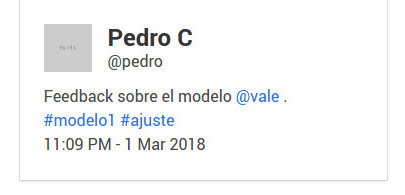
\includegraphics[width=7cm]{Img/UX/guia7.jpg}
    \centering
    \caption{\textbf{ \footnotesize{Tarjeta de comentario sobre un modelo.}}}
     \label{fig:comment}
    \end{figure}
    
    



\clearpage
\section{Producto Mínimo Viable y Experimentos}
Con las diferentes partes de las hipótesis definidas, se pueden determinar qué ideas sobre el producto son válidas y cuáles deben descartarse. El Producto Mínimo Viable (PMV) es muy importante porque si se prueban antes las funciones en las que merece la pena invertir, se pueden centrar los recursos de inmediato en las mejores soluciones. 


Esta es una de las maneras que tiene Lean UX para minimizar el despilfarro.
\begin{itemize}
    \item Primero se inicia con la lista de hipótesis priorizada.
    \item Luego, para determinar la validez de las declaraciones de hipótesis se crean los mínimos elementos posibles.
\end{itemize}
Esos elementos son los \textbf{PMV} que se utilizan luego para hacer experimentos. El resultado de esos experimentos indicará si la hipótesis fué correcta y si la dirección en la que se está trabajando es la indicada, debe perfeccionarse o debe abandonarse.

\begin{figure}[h]
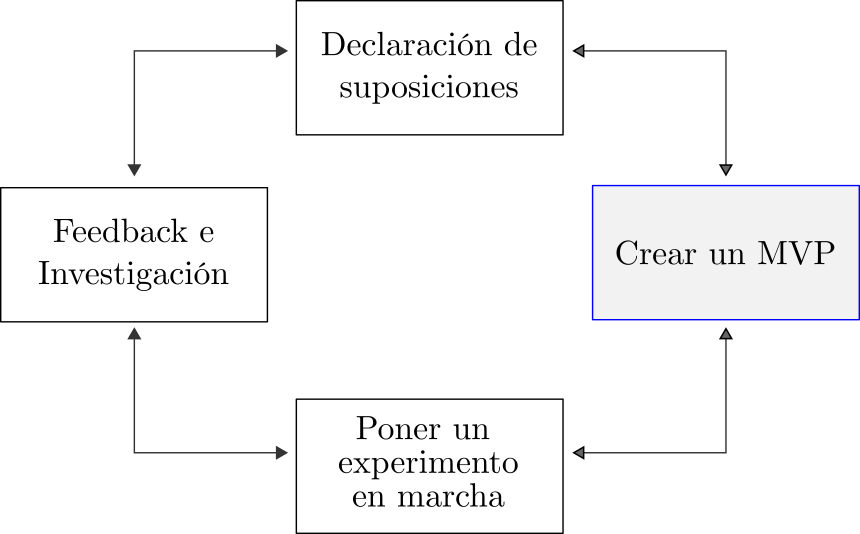
\includegraphics[width=10cm]{Img/Desarrollo/desarrollo2.png}
\centering
\caption{\textbf{ \footnotesize{Proceso LEAN UX, paso 2. }}}
\end{figure}
\label{fig:leanux2}

\subsection{Creación del PMV}
Al comenzar la planificación del PMV, lo primero que hay que tener en cuenta es lo que se quiere aprender con él. Por ello, resulta útil pensar estas tres cuestiones básicas: 
\begin{itemize}
    \item ¿Existe una necesidad para la solución que se diseña? 
    \item ¿Existe valor en la solución y las funciones que se ofrecen?
    \item  ¿La solución es usable?
\end{itemize}

Independientemente del propósito del PMV, esta etapa permite lanzar un producto y observar cómo interaccionan los usuarios con él en contextos realistas. Si con el PMV lo que se pretende es maximizar el aprendizaje, se debe:
\begin{itemize}
    \item Ser claro y conciso: dedicar el tiempo a depurar la idea hasta llegar a su proposición central de valor y presentar esa proposición a los usuarios. 
    \item Priorizar sin compasión: las ideas, como los artefactos, son pasajeras. Dejar que las mejores prueben su valor demostrando que aguantan el proceso de priorización. 
    \item Ser ágil: la información llega rápidamente, por lo que hay que asegurarse de durante el trabajo se pueda realizar actualizaciones con facilidad. 
    \item Medir el comportamiento: construir un PMV que permitan observar y medir lo que la gente hace realmente, no lo que dicen que hacen. En el diseño de productos digitales, el comportamiento es mucho más importante que las opiniones. 
    \item Utilizar una llamada-a-la-acción: se sabrá que el usuario valora la solución cuando demuestren que la usan.
\end{itemize}

\subsubsection{Creación del prototipo}
Una de las maneras más efectivas de crear los PMV es mediante un prototipo de la experiencia. \textit{Un prototipo es una aproximación de la experiencia de usuario que permite simular cómo será el uso del producto o servicio en cuestión}. Para que esa simulación sea efectiva deberá ser clicable (o bien tocarse con el dedo, dependiendo de la interfaz de usuario).
Por otra parte, como hay que dedicar el mínimo esfuerzo posible a su desarrollo, será importante que se elija bien la herramienta para crearlo. La elección de una herramienta u otra para el prototipo depende de: 
\begin{itemize}
    \item \textbf{¿Quién interactuará con él?} El primer prototipo lo utilizará el \textbf{usuario 1.b} establecido en la sección \ref{section:usuarios}: \textit{Personas que desean participar del proceso de diseño pero sin tener conocimientos sobre diseño 3D}.
    \item \textbf{¿Qué se espera aprender de él?} Se espera aprender aspectos de funcionalidad y usabilidad de la UI al momento de interactuar con un modelo 3D.
    \item \textbf{¿Cuánto tiempo se tiene para realizarlo?} Se cuenta con poco tiempo. Aproximandamente 4 días
\end{itemize}

\vspace{5mm}
\textbf{Desición del tipo de prototipo según la fidelidad}\vskip

\textit{La fidelidad se refiere al nivel de realismo en un prototipo}. Por ejemplo, un prototipo de baja fidelidad puede ser un boceto, en inglés \textit{sketch} dibujado a mano alzada sobre un papel, utilizando instrumentos de dibujo básicos como lápiz y goma de borrar. Un prototipo de alta fidelidad puede ser una herramienta de software que permita imitar el aspecto y el comportamiento de la interfaz real, las interfaces basadas en la web se pueden prototipar directamente con HTML y CSS, siendo posible reutilizar algunos fragmentos de código del prototipo en la interfaz real.\vskip
\textit{Mientras más alta sea la fidelidad del prototipo, más se aprende de él}. Por ejemplo, se aprenderá sobre qué colores funcionan mejor para atraer la atención y qué piensan los usuarios sobre el aspecto y la sensación del producto.
Si se ha desarrollado la guía de estilo, entonces es más fácil usar alta fidelidad porque no hay que pensar en la mayoría de las decisiones estéticas y se pueden enfocar los esfuerzos hacia las desiciones de funcionalidad.\vskip
A continuación, en la Figura \ref{fig:prototipo} se ilustra un gráfico de fidelidad en dos dimensiones con la elección de la herramienta para el prototipado. Sobre el eje de las abscisas se establecen los aspectos relacionados a la \textit{fidelidad visual} o bien qué tan parecido es estéticamente el prototipo respecto a la versión final, sobre el eje de las ordenadas se establecen los aspectos de \textit{fidelidad funcional} o que tan parecido se comporta el prototipo respecto a la versión final.

\vspace{5mm}
 \begin{figure}[h]
    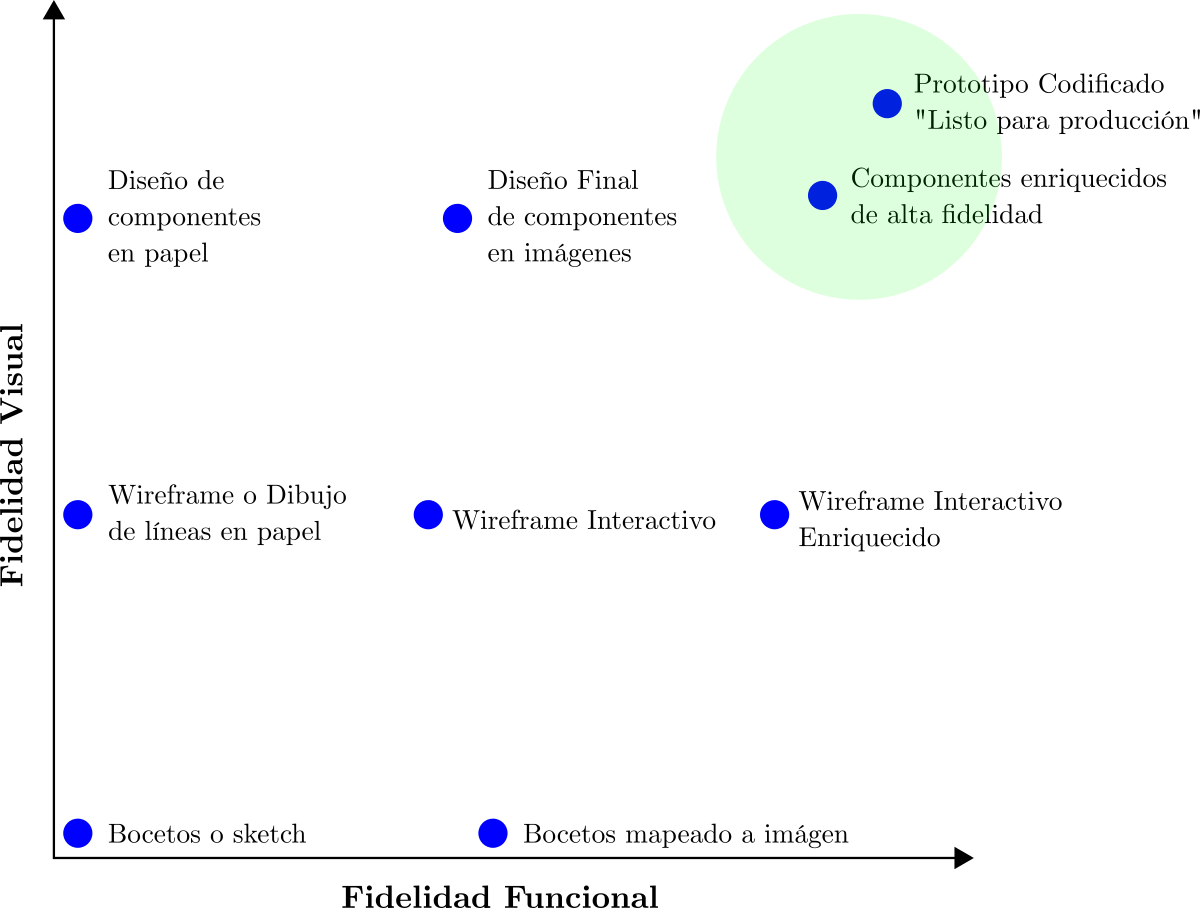
\includegraphics[width=14cm]{Img/UX/prototipo.png}
    \centering
    \caption{\textbf{ \footnotesize{Elección del tipo de prototipo}}}
    \label{fig:prototipo}
\end{figure}

Para este trabajo, se decide utilizar \textit{Prototipos de media y alta fidelidad} y \textit{Prototipos codificados}, como se puede observar en la parte superior derecha del gráfico. Las decisiones de funcionalidad se discuten en primera instancia mediante los bocetos en el \textit{estudio de diseño}. Los aspectos estéticos se establecen previamente en la guía de estilos.\vskip
Una vez elegida la herramienta para crear el PMV se inicia la construcción del prototipo, no es necesario incluir la experiencia de usuario completa del producto. En lugar de eso, se simula la parte más importante de esa experiencia. Se hace foco en los flujos de trabajo principales que ilustran el PMV. De esta manera el equipo puede observar una parte específica de la experiencia de usuario (tal y como será) para que puedan valorar su validez y su eficacia.

\subsection{Experimentos}

Se recomienda probar el PMV en primera instancia con los miembros del equipo, y luego con personas de otros equipos. Cuánto más se exponga el PMV a las miradas ajenas, más conocimiento se tendrá para validarlo. El siguiente paso será llevarlo a usuarios finales. Dejar que investiguen el prototipo y que lo utilicen libremente y así podrás obtener todo el feedback posible sobre la experiencia de usuario.

\begin{figure}[h]
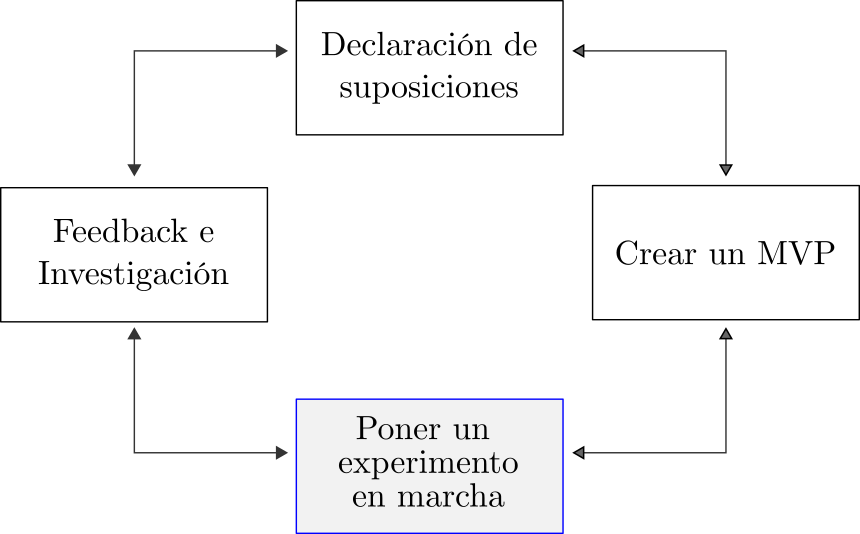
\includegraphics[width=10cm]{Img/Desarrollo/desarrollo3.png}
\centering
\caption{\textbf{ \footnotesize{Proceso LEAN UX, paso 3. }}}
\end{figure}
\label{fig:leanux3}

En la sección anterior se establece cuál es el primer prototipo para probar, en base al nivel de riesgo que implica su implementación (Si falla puede llevar el proyecto al fracazo). \vskip
\begin{itemize}
    \item \textbf{Usuario del experimento}. \textit{Personas que desean participar del proceso de diseño pero sin tener conocimientos sobre diseño 3D.
Se espera aprender aspectos de funcionalidad}
    \item \textbf{Qué se espera aprender con el experimento}. \textit{
    Se espera aprender aspectos de funcionalidad y usabilidad de la UI al momento de interactuar con un modelo 3D.}
\end{itemize}

    
Para realizar la primer prueba o experimento con el usuario final se utiliza una interfaz con un modelo 3D de ejemplo y sus respectivos parámetros para modificar la geometría y el color. Por convención, este experimento puede ser nombrado \textit{Demo \#1}, con el fin de establecer un orden en los experimentos. En la figura \refl{fig:feedback0} ilustra la pantalla inicial del Demo \#1 que se muestra al usuario.

Algunas características del experimento inicial son:
\begin{itemize}
    \item Se utiliza una computadora con el sistema operativo GNU/Linux y conexión a internet.
    \item Para acceder al prototipo se utiliza un navegador web con soporte de WebGL.
    \item El usuario no tiene que escribir ninguna URL, el prototipo aparece por defecto en la pantalla.
    \item El usuario no recibe instrucciones o capacitación de cómo utilizar el prototipo.
    \item No hay limites de tiempo para utilizar el prototipo.
\end{itemize}

\begin{figure}[h]
    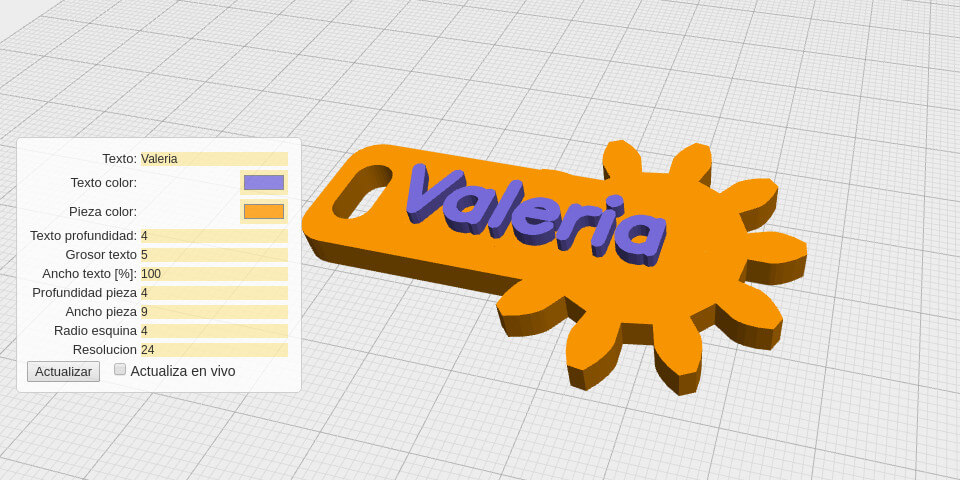
\includegraphics[width=14cm]{Img/Desarrollo/feedback0.jpg}
    \centering
    \caption{\textbf{ \footnotesize{Pantalla Inicial de Demo \#1}}}
     \label{fig:feedback0}
\end{figure}

El prototipo para la Demo \#1 se desarrolla en base al código de OpenJSCAD, adaptando algunas funcionalidades al usuario final. El desarrollo de este prototipo codificado es rápido, aproximadamente 36 horas. A continuación se señalan algunas ventajas y desventajas de el enfoque elegido para desarrollar este prototipo.\vskip

\textbf{Ventajas:}
\begin{itemize}
    \item Es posible reutilizar reutilizar su código en producción.
    \item Ofrecen la simulación más realista posible.
    \item Pueden generarse a partir de recursos existentes de código.
\end{itemize}

\textbf{Desventajas:}
\begin{itemize}
    \item Se puede perder mucho tiempo debatiendo sobre los detalles del prototipo.
    \item En muchos casos es necesario dedicar mucho tiempo a crear código funcional que muestre la experiencia deseada.
    \item Existe la tentación de perder tiempo perfeccionando el código antes de entregarlo a los clientes.
    \item En algunos casos, la actualización y la iteración pueden llevar mucho tiempo.
\end{itemize}

\clearpage
\section{Feedback e Investigación}
En esta instancia se debe probar el PMV desarrollado. Hasta ahora, todo el trabajo esta basado en las suposiciones; a partir de este punto se comienza con el proceso de validación. Se Utilizan técnicas de investigación ligeras, continuas y colaborativas para hacerlo. La investigación con usuarios, se encuentra en el centro de la mayoría de las estrategias de la experiencia de usuario. Un error común es realizar esta investigación solo a veces, normalmente al principio del proyecto o al final. Lean UX resuelve estos problemas convirtiendo la investigación en algo continuo y colaborativo.

Lean UX toma las técnicas de investigación de mercado de UX, uniendo dos ideas importantes. En primer lugar, la investigación con esta metodología es continua, lo que significa que estas actividades se realizan en cada \textit{sprint del producto}. En lugar de poner en marcha un proceso costoso y largo, que interrumpe el proceso de diseño, la investigación se realiza en pequeñas partes, de manera que encaje bien con el proceso de diseño en marcha. En segundo lugar, la investigación de Lean UX es colaborativa: no es necesario utilizar el trabajo empresas externas especializadas para que el equipo pueda aprender sobre el comportamiento de sus clientes. Las responsabilidades de esta labor son responsabilidad de todo el equipo y se comparten entre todos. El objetivo de todo este proceso es crear un conocimiento compartido entre todos los miembros del equipo. 

\begin{figure}[h]
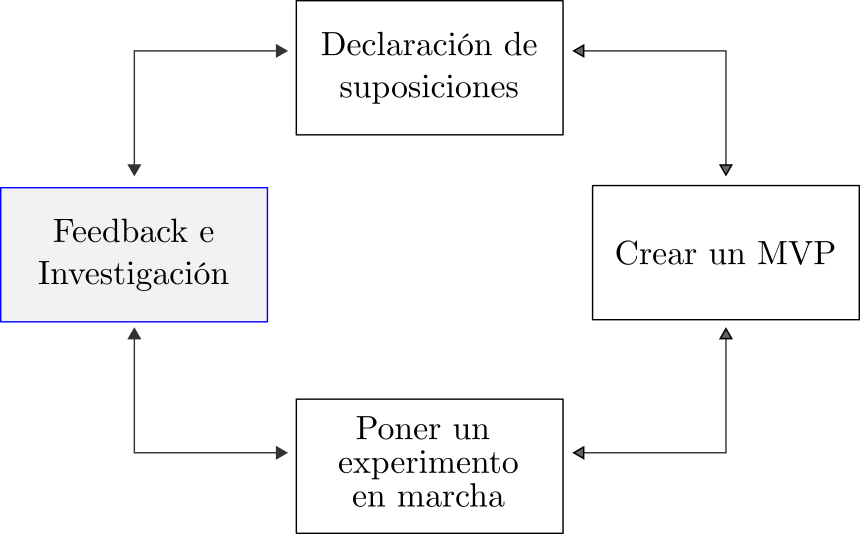
\includegraphics[width=10cm]{Img/Desarrollo/desarrollo4.png}
\centering
\caption{\textbf{ \footnotesize{Proceso LEAN UX, paso 4. }}}
\end{figure}
\label{fig:leanux4}

\clearpage
El descubrimiento colaborativo es una manera de conseguir que todo el equipo haga trabajo de campo. Una buena práctica que resulta crítica para Lean UX es la implicación regular de los usuarios con el producto. Las conversaciones con los usuarios, según un calendario especificado previamente, minimizan el tiempo que transcurre entre la creación de las hipótesis, el diseño de los experimentos y el feedback de los usuarios, con lo que resulta posible validar rápidamente las hipótesis. En general, saber que el feedback de los usuarios se realiza regularmente tiene un poderoso efecto sobre los equipos, ya que les quita presión a la hora de tomar decisiones. A fin de cuentas, saben que en pocos días dispondrán de datos significativos obtenidos directamente del contexto real en el que se utilizará el producto.

\subsection{Feedback con el usuario}
Una vez que se enseña el PMV y se deja que el cliente interactué con él. Es recomendable tomar notas a medida que el cliente vaya dando su opinión. Al final de la entrevista o sesión de prueba, se pide referencias al cliente de otras personas que podrían encontrar útil el producto.

A continuación se realizan una serie de preguntas sobre la experiencia de usuario en el uso de la interfaz gráfica UI. 
Para obtener un aprendizaje más específico, las preguntas se dividen en tópicos relacionados a diferentes aspectos de funcionalidad. A continuación se enumeran los tópicos a evaluar en el Demo \#1:
\begin{enumerate}
    \item Visualización del modelo 3D
    \item Zoom (Aumentar, reducir)
    \item Rotación (Girar)
    \item Translación (Mover)
    \item Modificación de parámetros
\end{enumerate}
Las respuestas posibles son Buena, Regular o Mala. En caso de responder Regular o Mala se realiza otras 2 preguntas: ¿Cual es el inconveniente inconveniente? y ¿Qué sugiere para resolver ese inconveniente?

En la tabla siguiente se especifican los resultados del feedback para Demo \#1:


\begin{tabular}{ |p{0.8cm}|p{2.3cm}|p{2.2cm}|p{3.6cm}|p{3.6cm}| }
\hline
     Ítem & Tópico & Experiencia  & Inconveniente & Cómo mejorar\\
\hline
1 & Visualización & Buena & - & -\\
\hline
2 & Zoom & Regular & Al hacer demasiado zoom sobre el modelo ocurre que no hay un limite, lo que produce que se vea rota la geometría. & Limitar el zoom o ver la posibilidad de volver la visualización a su estado original, como se muestra al inicio de la sesión.\\
\hline
2 & Rotación & Buena & - & -\\
\hline
3 & Translación & Mala & Al mover demasiado la pieza y haciendo zoom sobre el modelo ocurre que se pierde la visualización y parece que la escena esta vacía. & Limitar la opción de mover o ver la posibilidad de volver la visualización a su estado original, como se muestra al inicio de la sesión.\\
\hline
4 & Modificación de parámetros & Regular & No es cómodo cargar números en los campos por medio del teclado & Agregar un elemento parecido a los que tienen las apps.\\
\hline
\end{tabular}

\subsection{Análisis de resultados del feedback}
Efectivamente el feedback con el usuario se traduce en la obtención de inconvenientes en la funcionalidad (desde su punto de vista) que no pudieron ser detectados en las pruebas con el equipo. La incapacidad de detectar errores por parte del equipo se debe muchas veces a que el equipo ya conoce el funcionamiento del producto y por ende se limita a utilizarlo en condiciones acotadas por ese conocimiento. A continuación se pueden apreciar visualmente los errores encontrados por el usuario y un breve análisis sobre el feedback en cada topico.

\begin{enumerate}
    \item Visualización del modelo 3D. Ningún inconveniente, el usuario tiene una experiencia de uso positiva.
    \item Zoom (Aumentar, reducir). En la Figura \ref{fig:feedback1} se puede apreciar este inconveniente, sobre todo en la parte donde se ``rompe" la geometría al aumentar el zoom muy cerca de la modelo. Si bien, se puede resolver reduciendo el zoom o alejándose de la escena, no se visualiza en la interfaz mecanismo inmediato para salir de esta situación. El usuario tiene una experiencia de uso negativa.
    \item Rotación (Girar). Ningún Inconveniente, el usuario tiene una experiencia de uso positiva.
    \item Translación (Mover). En la Figura \ref{fig:feedback2} se puede apreciar que el modelo prácticamente desaparece de la pantalla al moverlo y hacer zoom sobre otra área de la escena. No se visualiza en la interfaz un mecanismo inmediato para salir de esta situación. El usuario tiene una experiencia de uso negativa.
    \item Modificación de parámetros. La mayoria de los usuarios en la actualidad están acostumbrados a las interfaces con componente gráficos como deslizadores en los que no es necesario escribir los valores numéricos. En la Figura \ref{fig:feedback3} se puede apreciar la ausencia de este tipo de elementos. El usuario tiene una experiencia de uso negativa.
\end{enumerate}


\begin{figure}[h]
    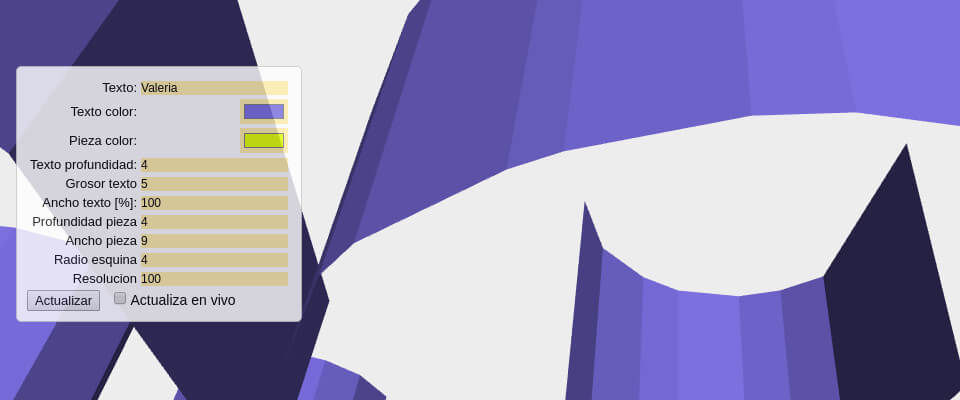
\includegraphics[width=16cm]{Img/Desarrollo/feedback2.jpg}
    \centering
    \caption{\textbf{ \footnotesize{Inconvenientes con el zoom en Demo \#1}}}
     \label{fig:feedback1}
\end{figure}

\begin{figure}[h]
    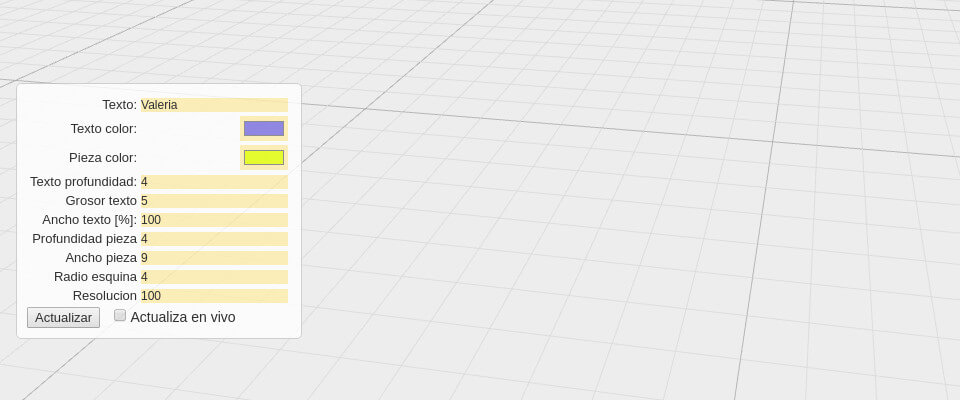
\includegraphics[width=16cm]{Img/Desarrollo/feedback3.jpg}
    \centering
    \caption{\textbf{ \footnotesize{Inconvenientes con la translación en Demo \#1}}}
     \label{fig:feedback2}
\end{figure}

\begin{figure}[h]
    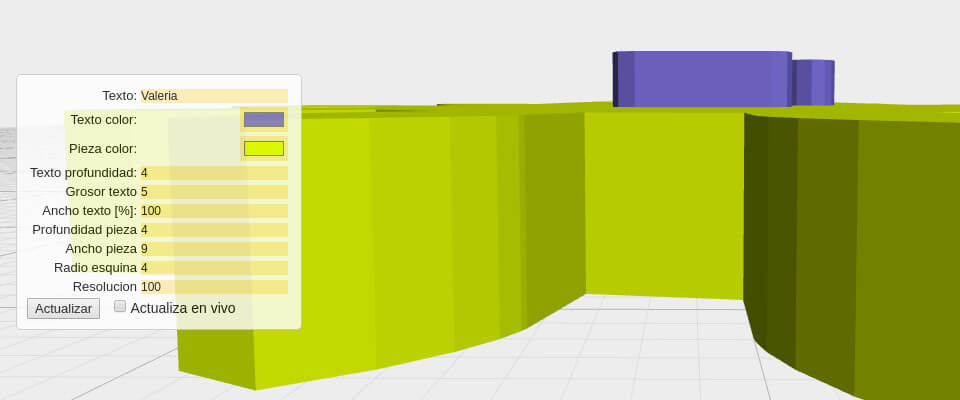
\includegraphics[width=16cm]{Img/Desarrollo/feedback1.jpg}
    \centering
    \caption{\textbf{ \footnotesize{Inconvenientes con la carga de parametros en Demo \#1}}}
     \label{fig:feedback3}
\end{figure}

\clearpage
\section{Definicion del sistema}
https://nuxtjs.org/guide#what-is-nuxt-js-

#\subsection{Mockup}

#\subsection{One Page / Single-page application}
http://1.droppdf.com/files/A32RR/manning-single-page-web-applications-javascript-end-to-end-2014.pdf

#(https://theseus.fi/bitstream/handle/10024/97217/Kokkonen_Juha.pdf?sequence=1 ,pag 9)

#Las aplicaciones web de una sola página proporcionan una experiencia similar a las de escritorio en un navegador web estandar. 

#\subsection{Programación Reactiva}
#\subsection{Programación Reactiva (Manifiesto)}
(traducción en odt)
#\begin{itemize}
#\item Responsivo:
#\item Resiliente:
#\item Elástico:
#\item Dirigido por Mensajes:
#\end{itemize}
#\subsection{Relación entre el patrón de diseño observable y la Programación Reactiva}
(en vuejs odt)
#\subsection{--FrontEnd--}
#\subsection{vue.js}
guia español: https://es-vuejs.github.io/vuejs.org/v2/guide/

#rendimiento vue
https://www.kairosds.com/blog/vue-js-exito/

#\subsection{Guías de estilo: Bulma}
#\subsection{nuxt.js}

#Traduciendo libremente la explicación que aparece en la página de nuxt.js:

    El 25 de octubre de 2016, el equipo detrás de zelt.co, anuncia Next.js, un framework para aplicaciones React renderizadas en el lado servidor. Pocas horas después de ese anuncio, la idea de crear aplicaciones renderizadas del lado servidor en Vue.js de la misma forma que Next.js era obvia. Nuxt.js había nacido.
https://www.opsou.com/es/blog/nuxtjs-una-pieza-mas-del-ecosistema-vuejs-introduccion


#Nuxt.js es un framework para crear aplicaciones universales en Vue.js. Una aplicación universal es aquella que su código puede ser ejecutado tanto en el cliente como en el servidor. Nuxt.js tiene muchas características, pero una de las más interesantes es que nos ayuda a crear aplicaciones Vue.js que se renderizan del lado del servidor (SSR – Server-Side Rendering). Esto quiere decir que se precargan las páginas en el servidor y luego se envía el HTML renderizado al navegador.
https://www.groloop.com/vue-js-2-12-aplicaciones-vue-js-universales-con-nuxt-js/

#Una aplicación universal es aquella que comparte todo (o casi todo) su código entre el cliente y el servidor.
https://medium.com/@sergiodxa/qu%C3%A9-es-una-aplicaci%C3%B3n-universal-f1258d030f25

#ventajas y desventajas
https://github.com/i62navpm/Tutorial-Nuxt

#\subsection{--Backend--}
#\subsection{node.js}
#\subsection{express}
#\subsection{API RESTFUL}
#ver PDF: API REST y sistema de aprovisionamiento en containers para servIoTicy

#book: https://www.amazon.es/RESTful-API-Design-Practices-API-University-ebook/dp/B01L6STMVW

#Tesis Doctoral: #http://www.ics.uci.edu/~fielding/pubs/dissertation/rest_arch_style.htm
Artículo: https://www.infoq.com/articles/subbu-allamaraju-rest
Book: https://pages.apigee.com/rs/apigee/images/api-design-ebook-2012-03.pdf (ver fuentes)
Book: https://doc.lagout.org/programmation/Webservers/REST%20API%20Design%20Rulebook%20-%20Masse%20-%20O%27Reilly%20%282012%29/REST%20API%20Design%20Rulebook%20-%20Masse%20-%20O%27Reilly%20%282012%29.pdf

#Consideraciones de diseño 
  - no verbos
  - url en minuscula, no usar _ 
  - usar uri
  
#Metodos get/post/delete/etc

#\subsection{ORM: sequelize}
http://docs.sequelizejs.com/

#\subsection{--test--}
#\subsection{¿Framework para test?}


#\section{MVP - Prototipado}
#\subsection{Prototipado rápido HTML más Bulma}

#\begin{figure}
#\centering
#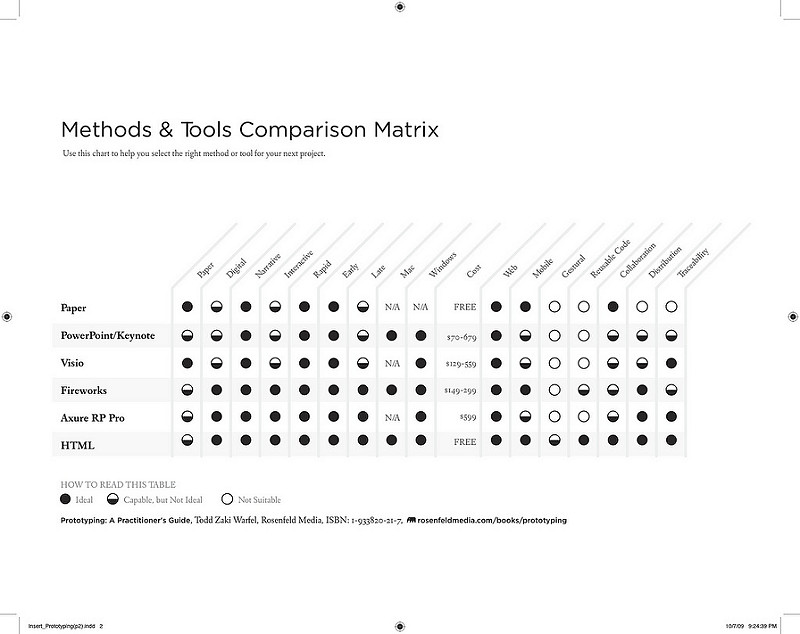
\includegraphics[width=16cm]{Img/UX/UX-matrix.jpg}
#\caption[Proto-persona (optional short caption)]{\label{us_figure} Matriz de herramientas para prototipado. Extender a nuevas herramientas}
#\end{figure}

#\section{Herramientas tecnológicas para el desarrollo}

#\subsection{Lenguaje Ubicuo: De Historias a Escenarios y tests}

Scenario: Listar los Trabajos\vskip0mm
  Given: Estoy en URL\vskip0mm
  Then: Veo el título "Pieza de Pruebas"\vskip10mm
 
Scenario: Acceder al Escritorio de Trabajo\vskip0mm
  Given: Estoy en URL\vskip0mm
  When: Hago click en "Pieza de Pruebas"\vskip0mm
  Then: Estoy en URL\vskip0mm
  Then: Veo el título "Pieza de Pruebas"\vskip0mm
  And: Veo la etiqueta "Alto"\vskip0mm
  And: Veo la etiqueta "Ancho"\vskip0mm
  And: Veo la etiqueta "Profundidad"\vskip0mm
  And: Veo el Visor de la Pieza "stl-view"
  
#\subsection{Especificación BDD Escenarios, Cucumber, etc}

#\subsection{Programación SPA (Single Page App)}

#\begin{displayquote}
An SPA is an application delivered to the browser that doesn’t reload the page during use. Like all applications, it’s intended to help the user complete a task, such as “write a document” or “administer a web server.” We can think of an SPA as a fat client that’s loaded from a web server. \cite{Mikowski2015}
#\end{displayquote}

#\say{The single-page web interface is composed of individual components which can be updated/replaced independently, so that the entire page does not need to be reloaded on each user action.\cite{Mesbah2007}}


#\subsection{Visualización y datos (WebGL, OpenJSCAD)}

#\subsection{Frontend Vue.js}

#\subsection{Backend (Node.js, Express, GraphQL, ES 2015 )}


#\section{Métricas, ecuaciones, fórmulas, posibilidades}


#\section{Construcción del sistema}

#\subsection{Modelado de Classes}

#\subsection{Diseño y Código en JS (FLUX?)}

#\subsection{API: GraphQL}


#\section{Funcionalidades}

#\subsection{Control de versiones}

#\subsection{Integración con otras plataformas (embed)}

#\subsection{Compartir proyectos (share)}

#\subsection{Exportar modelos}

#\subsection{Extras: Anotaciones, comentarios, adjuntar imagen, chat, etc}



#\section{Descripción general del prototipo}
El prototipo de entorno colaborativo cuenta con una arquitectura que permite desplegar un aplicación multiplataforma accesible a través de un navegador web.

Está conformado por 2 componentes de software.
El primer componente se denomina Capa de Servicios (Backend) y es una aplicación de servidor que permite:
\begin{itemize}
  \item Iniciar y parar los servicios. 
  \item Conocer el estado de los servicios.
  \item Guardar registros de bitácora (LOGS).
  \item Gestionar peticiones de los clientes.
  \item Exponer la interfaz de usuario (Segundo componente).
\end{itemize}

El segundo componente es una interfaz construida con tecnologías web (Front-End) y se ejecuta en un navegador web convencional, permitiendo al usuario:
\begin{itemize}
  \item Visualizar un modelo 3D con funciones de acercamiento (zoom), rotación y translación.
  \item Compartir el entorno colaborativo mediante un hiperenlace web.
  \item Visualizar y Manipular parámetros relacionados al modelo 3D de manera sencilla e intuitiva.
  \item Agregar información extra (anotaciones, imágenes, etc) relacionados al modelo.
  \item Generar nuevas versiones de los modelos en un mismo espacio de trabajo.
  \item Explorar todas las versiones y los cambios de parámetros respecto a su antecesor.
  \item Recibir notificaciones referente a las acciones de otros usuarios sobre el entorno.
 
\end{itemize}

